\section{Rust 開発環境を設定する}

Rust 開発環境を設定し、プログラムを記述し、Cargo ビルド システムを使用する方法について説明します。

\subsection{学習の目的}

このモジュールでは、次の方法を学習します。

\begin{itemize}
\item Rust を使用するための開発環境を設定します。
\item 単純な "Hello World" プログラムを 作成します。
\item Rust のビルド ツールであり、依存関係マネージャーである Cargo を使用します。
\end{itemize}



\subsection{はじめに}

このユニットでは、Rust でのプログラミングを開始できるよう、開発環境をインストールして構成する手順について説明します。

Rust でプログラミングするには、Visual Studio Code エディター、Visual Studio Code 用 Microsoft C++ ビルド ツール、Rust 言語ファイルをインストールします。

環境を設定したら、基本的な "Hello World!" プログラムを試して、 次に進む準備ができたかを確認します。

\subsubsection{学習の目的}

このモジュールでは、次の方法を学習します。

\begin{itemize}
Rust を使用するように開発環境を設定します。
基本的な "Hello World!" をコンパイルして実行します 作成します。
Rust のビルド ツールであり、依存関係マネージャーである Cargo を使用します。
\end{itemize}
 % はじめに
\subsection{Visual C++ ビルド ツールをインストールする}

Rust には、Visual Studio 2013 以降の Microsoft C++ ビルド ツールが必要です。 Rust をインストールするには、事前にこれらのビルド ツールがインストールされている必要があります。

ビルド ツールがインストールされていない場合は、次の手順に従います。


\begin{enumerate}
\item Microsoft Visual Studio Code のダウンロード ページにアクセスします。

\item $[$Build Tools のダウンロード] を選択します。

\item ダウンロードが完了したら、インストーラー ファイルを実行します。 Visual Studio インストーラー ウィンドウが開きます。

\item ポップアップ ダイアログで、[はい] を選択します。 次のポップアップ ダイアログで、[続行] を選択します。

\item インストーラー ウィンドウの [デスクトップとモバイル] で、左側にある [C++ Build Tools] オプションのチェックボックスをオンにします。

\item 右側の [インストールの詳細] ウィンドウで、次のオプションが選択されていることを確認します。
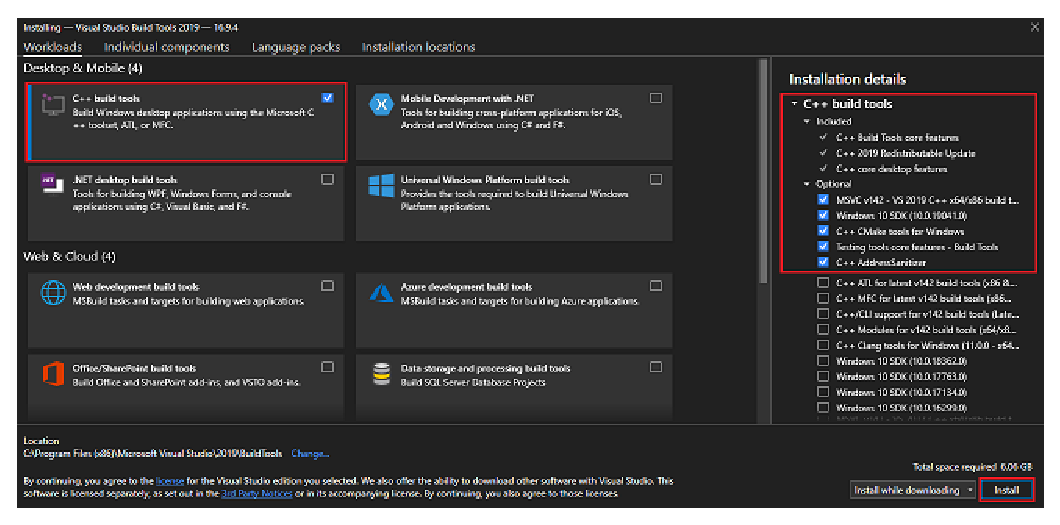
\includegraphics[width=14cm]{install-visual-cpp-build-tools.eps}

\item 右下にある [インストール] を選択します。
\end{enumerate}

インストールが完了したら、Rust のインストールを続行できます。
 % Visual Studio Code をインストールする
\subsection{Visual C++ ビルド ツールをインストールする}

Rust には、Visual Studio 2013 以降の Microsoft C++ ビルド ツールが必要です。 Rust をインストールするには、事前にこれらのビルド ツールがインストールされている必要があります。

ビルド ツールがインストールされていない場合は、次の手順に従います。


\begin{enumerate}
\item Microsoft Visual Studio Code のダウンロード ページにアクセスします。

\item $[$Build Tools のダウンロード] を選択します。

\item ダウンロードが完了したら、インストーラー ファイルを実行します。 Visual Studio インストーラー ウィンドウが開きます。

\item ポップアップ ダイアログで、[はい] を選択します。 次のポップアップ ダイアログで、[続行] を選択します。

\item インストーラー ウィンドウの [デスクトップとモバイル] で、左側にある [C++ Build Tools] オプションのチェックボックスをオンにします。

\item 右側の [インストールの詳細] ウィンドウで、次のオプションが選択されていることを確認します。
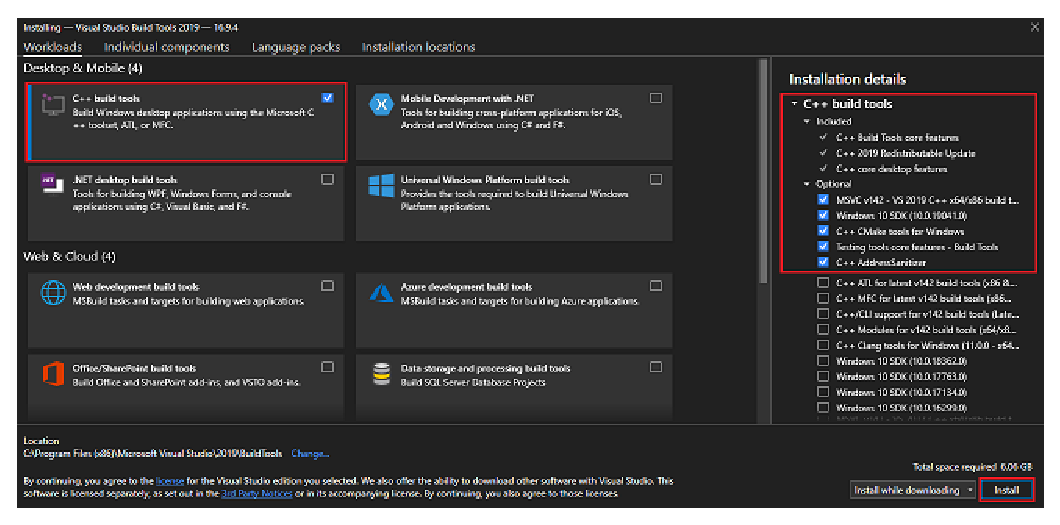
\includegraphics[width=14cm]{install-visual-cpp-build-tools.eps}

\item 右下にある [インストール] を選択します。
\end{enumerate}

インストールが完了したら、Rust のインストールを続行できます。
 % Visual C++ ビルド ツールをインストールする
\subsection{Rust をインストールする}

Rust をインストールするために推奨される方法は、Rust ツールチェーン インストーラーの \texttt{rustup} を使用することです。 Web サイト rustup.rs にアクセスして、お使いのオペレーティング システムに合った手順を見つけてください。

\includegraphics[width=10cm]{rustup.eps}

Linux または macOS 上では、クリップボード アイコンを選択して curl コマンドをコピーします。 次に、コンピューターのターミナルまたはコマンド プロンプトを開いてコマンドを貼り付け、画面の指示に従います。 Windows 上では、インストーラーの指示に従います。

\begin{itembox}[l]{重要}
Rust には、Visual Studio 2013 以降の Microsoft C++ ビルド ツールが必要です。 Rust をインストールするには、事前にビルド ツールがインストールされている必要があります。 ビルド ツールをインストールする必要がある場合は、前のユニットの手順を参照してください。
\end{itembox}

Rust のラピッド リリース プロセスは 6 週間ごとに実行されます。非常に多くのプラットフォームがサポートされているので、任意の時点で利用できる Rust のビルドは多数存在します。 \texttt{rustup} を以前にインストールしたことがある場合は、\texttt{rustup update} コマンドを実行することで、Rust の最新の安定バージョンに更新できます。

\subsubsection{Rust のインストールを確認する}

Rust のインストールを完了したら、\texttt{rustc} コマンドと \texttt{cargo} コマンドを使用できるようになります。

\begin{itembox}[l]{注意}
次のコマンドはすべてのプラットフォームで動作します。
\end{itembox}

ターミナルまたはコマンド プロンプトで、次のコマンドを実行します。


\begin{lstlisting}[numbers=none]
rustc --version
\end{lstlisting}

この例のような出力になるはずです。

\begin{lstlisting}[numbers=none]
rustc 1.50.0 (cb75ad5db 2021-02-10)
\end{lstlisting}

次に、次のコマンドを実行します。

\begin{lstlisting}[numbers=none]
cargo --version
\end{lstlisting}

次のような出力が表示されます。

\begin{lstlisting}[numbers=none]
cargo 1.50.0 (f04e7fab7 2021-02-04)
\end{lstlisting}

いずれの出力行にも、利用可能な Rust と Cargo の最新の安定したバージョンに関する次の情報が含まれます。

\begin{itemize}
\item リリース番号
\item コミット ハッシュ
\item コミットの日付
\end{itemize}

この情報は次の形式で表示されます。

\texttt{<executable-name> <three-part-release-number> (<9-character-hash-code> <4-digit-year>-<2-digit-month>-<2-digit-day>)}

この種類の出力が表示された場合、両方のインストールが成功しました。 この情報が表示されない場合、\texttt{PATH} 環境変数を確認してください。 \texttt{rustc.exe} と \texttt{cargo.exe} という実行可能ファイルが入っているフォルダーが必ず含まれるようにしてください。

\subsubsection{自分の知識をチェックする}

次の質問に答えて、学習した内容を確認してください。

\begin{enumerate}
\item Rust のインストールに使用するために推奨されているコマンドは何ですか?

\begin{itemize}
\item rinstall
\item rustup
\item rupdate
\end{itemize}

\item Rust ライブラリはどのくらいの頻度で更新されますか?
\begin{itemize}
\item 6 か月ごと
\item 3 か月ごと
\item 6 週間ごと
\end{itemize}
\end{enumerate}

 % Rust をインストールする
\subsection{演習: Hello World}

Rust がインストールされていれば、コーディングを開始する準備ができています。 "Hello, world!" を出力するプログラムを作成しましょう。 コンソールに表示します。

\subsubsection{コードを整理するための新しいディレクトリを作成する}

このラーニング パス (\texttt{rust-learning-path}) のすべてのコードを格納するディレクトリを作成することから始め、その後、この演習のソース コードを保存するための新しいサブディレクトリを作成します。

Linux、macOS、および Windows 上の PowerShell の場合は、次のコマンドを実行します。

\begin{lstlisting}[numbers=none]
mkdir ~/rust-learning-path
cd ~/rust-learning-path
mkdir hello-world
cd hello-world
\end{lstlisting}

\subsubsection{最初の Rust プログラムを記述する}

次に、\texttt{main.rs} という名前の新しいファイルを作成し、エディターを使用して次のコードを記述します。

\begin{lstlisting}[numbers=none]
fn main() {
    println!("Hello, world!");
}
\end{lstlisting}

\subsubsection{プログラムをコンパイルして実行する}

ソース コードの準備ができました。 次に、プログラムをコンパイルして実行可能ファイルを作成します。 ターミナル ウィンドウに戻り、次のコマンドを入力して、ファイルをコンパイルして実行します。

Linux または macOS を使用している場合は、次のコマンドを実行します。


\begin{lstlisting}[numbers=none]
rustc main.rs
./main
\end{lstlisting}

次の出力が表示されます。

\begin{lstlisting}[numbers=none]
Hello, world!
\end{lstlisting}

\subsubsection{Cargo を使用してプロジェクトを作成する}

ここで、Cargo を使用して、同じプログラムを記述して実行しましょう。

\begin{itembox}[l]{注意}
次のセクションのコマンドはすべてのプラットフォームで動作します。
\end{itembox}

まず、Cargo を使用して新しいプロジェクトを作成します。

ターミナルが \texttt{rust-learning-path} ディレクトリにあることを確認し、次のコマンドを実行します。


\begin{lstlisting}[numbers=none]
cargo new hello-cargo
\end{lstlisting}

このコマンドにより、hello-cargo という名前の新しいディレクトリが src サブディレクトリと共に生成され、次の 2 つのファイルが追加されます。

\begin{lstlisting}[numbers=none]
hello-cargo/
     Cargo.toml
     src/
         main.rs
\end{lstlisting}

\begin{itemize}
\item Cargo.toml ファイルは、Rust のマニフェスト ファイルです。 プロジェクトのメタデータとすべての依存関係をここに保存します。
\item src サブディレクトリの main.rs ファイルは、アプリケーション コードを記述する場所です。
\end{itemize}

\texttt{cargo new} コマンドによって、"Hello, world!" という定型句が 生成されました。

\subsubsection{Cargo を使用してプログラムをビルドして実行する}

この定型プログラムを実行するには、新しいディレクトリ hello-cargo に移動し、\texttt{cargo run} コマンドを使用します。

ターミナルで次のコマンドを実行します。


\begin{lstlisting}[numbers=none]
cd hello-cargo
cargo run
\end{lstlisting}

次のような出力がターミナルに表示されます。

\begin{lstlisting}[numbers=none]
  Compiling hello-cargo v0.1.0 (/tmp/.OFUp/hello-cargo)
    Finished dev [unoptimized + debuginfo] target(s) in 1.59s
      Running `target/debug/hello-cargo`

Hello, world!
\end{lstlisting}

Cargo により、実行可能ファイルがビルドされ、実行されました。

お疲れさまでした。これで最初の Rust プログラムを記述し、Cargo を使用して最初の Rust プロジェクトを初期化する方法を学習しました。






 % 演習: Hello World
\subsection{まとめ}

このモジュールでは、Rust と、Rust プログラムを記述して実行するために必要な Visual Studio Code ツールをインストールしました。 環境を設定した後に、基本的な "Hello World!" プログラムをビルドし、Cargo を使用して新しいプロジェクト テンプレートを開始するように変更しました。

このラーニング パスの次のモジュールでは、関数、データ型、制御フローなど、Rust のいくつかの一般的なプログラミング概念について学習します。 % まとめ

